\chapter{动物分类}\label{ch:g4:classifying-animals}

自然历史博物馆收藏着数以百万计的\omterm{def:g1:animals-around-us:animal}{动物}——整屉的甲虫、
整厅的\omterm{def:g3:bones-and-muscles:skeleton}{骨骼}、整罐的鱼。然而，馆长几分钟之内
就能找到其中任何一件。秘诀不在记忆，而在于\emph{秩序}：
每种\omterm{def:g1:animals-around-us:animal}{动物}都在一个庞大的系统中占有自己的位置，
这个系统由\omterm{def:g4:classifying-animals:classification}{层层嵌套的类群}构成，依据的是
\cref{ch:g3:sorting-living-things}中的\omterm{def:g4:classifying-animals:classification}{分类}规则——
而今年我们将学习这个系统如何运作。

\section{层层嵌套的类群}

\begin{definition}[分类]\label{def:g4:classifying-animals:classification}
对\omterm{def:g1:living-or-not:living}{生物}进行\emph{分类}\index{分类}，就是依据共有的身体特征，
把它们归入不同的类群，再把这些类群归入
更大的类群——\emph{层层嵌套的类群}\index{层层嵌套的类群}，
就像盒子里套盒子。整个
这种排列就是一个\emph{分类}\index{分类}。
\end{definition}

\begin{example}[猫的分类地址]\label{ex:g4:classifying-animals:cat}
一只猫有好几重嵌套的“地址”：猫是一种\emph{\omterm{prop:g3:sorting-living-things:groups}{哺乳动物}}
（有\omterm{def:g1:animals-around-us:covering}{皮毛}，幼体靠\omterm{def:g2:animals-grow-up:born}{乳汁}哺育）；每一种\omterm{prop:g3:sorting-living-things:groups}{哺乳动物}都是一种
\emph{\omterm{def:g4:classifying-animals:vertebrate}{脊椎动物}}（体内有\omterm{def:g3:bones-and-muscles:skeleton}{骨骼}和\omterm{def:g4:classifying-animals:vertebrate}{脊柱}）；每一种\omterm{def:g4:classifying-animals:vertebrate}{脊椎动物}都是
一种\emph{\omterm{def:g1:animals-around-us:animal}{动物}}。猫在\omterm{prop:g3:sorting-living-things:groups}{哺乳动物}之中，\omterm{prop:g3:sorting-living-things:groups}{哺乳动物}
在\omterm{def:g4:classifying-animals:vertebrate}{脊椎动物}之中，\omterm{def:g4:classifying-animals:vertebrate}{脊椎动物}在\omterm{def:g1:animals-around-us:animal}{动物}之中：每个盒子
都套在一个更大的盒子里。
\end{example}

\begin{definition}[脊椎动物与无脊椎动物]\label{def:g4:classifying-animals:vertebrate}
\emph{脊椎动物}\index{脊椎动物}是体内有\omterm{def:g3:bones-and-muscles:skeleton}{骨骼}的\omterm{def:g1:animals-around-us:animal}{动物}，
其\omterm{def:g3:bones-and-muscles:skeleton}{骨骼}以\emph{脊柱}\index{脊柱}为中轴——
就像你在\cref{ex:g3:bones-and-muscles:feel}中摸到的脊柱。
没有脊柱的\omterm{def:g1:animals-around-us:animal}{动物}则称为
\emph{无脊椎动物}\index{无脊椎动物}：\omterm{prop:g3:sorting-living-things:groups}{昆虫}、蜘蛛、
蜗牛、蠕虫、水母——占所有\omterm{def:g1:animals-around-us:animal}{动物}的绝大多数。
\end{definition}

\begin{omfigure}
\begin{tikzpicture}[scale=0.86]
  % outer box: animals
  \draw[thick, omExo] (-0.3,-0.5) rectangle (12.1,4.4);
  \node[font=\small\bfseries, omExo] at (0.9,4.1) {动物};
  % vertebrates box
  \draw[thick, omDef, fill=omDef!4] (0.0,-0.2) rectangle (7.4,3.6);
  \node[font=\small\bfseries, omDef] at (1.35,3.3) {脊椎动物};
  \node[font=\footnotesize, omDef] at (2.6,2.85) {（体内有脊柱）};
  % five classes
  \foreach \x/\name in {0.25/鱼类, 1.65/两栖动物, 3.05/爬行动物,
      4.45/鸟类, 5.85/哺乳动物} {
    \draw[thick, omMeth, fill=omMeth!7] (\x,0.1) rectangle ({\x+1.3},2.4);
    \node[font=\footnotesize, rotate=90] at ({\x+0.65},1.25) {\name};
  }
  % invertebrates box
  \draw[thick, omProp, fill=omProp!5] (7.8,-0.2) rectangle (11.9,3.6);
  \node[font=\small\bfseries, omProp] at (9.2,3.3) {无脊椎动物};
  \node[font=\footnotesize, align=center] at (9.85,1.4)
    {昆虫、蜘蛛、\\ 蜗牛、蠕虫、\\ 水母、\dots\\[3pt]
     （绝大多数动物！）};
\end{tikzpicture}

{\small 盒子套盒子：\omterm{def:g4:classifying-animals:vertebrate}{脊椎动物}的五个纲合在一起
构成一个盒子，与数量多得多的\omterm{def:g4:classifying-animals:vertebrate}{无脊椎动物}并排，
同处于所有\omterm{def:g1:animals-around-us:animal}{动物}的盒子之中。}
\end{omfigure}

\section{脊椎动物的五个纲}

\begin{proposition}[脊椎动物的五个纲]\label{prop:g4:classifying-animals:classes}
\omterm{def:g4:classifying-animals:vertebrate}{脊椎动物}被划分为五大类群，称为
\emph{纲}\index{纲（脊椎动物）}：
\begin{enumerate}
  \item \emph{\omterm{prop:g3:sorting-living-things:groups}{鱼类}}：鳞片、鳍，在水中呼吸——鳟鱼、
        鲨鱼、沙丁鱼；
  \item \emph{两栖动物}\index{两栖动物}：\omterm{def:g1:the-five-senses:sense}{皮肤}湿润裸露，
        卵产在水中，经历\omterm{ex:g2:animals-grow-up:frog}{蝌蚪}期——青蛙、蟾蜍、蝾螈；
  \item \emph{爬行动物}\index{爬行动物}：\omterm{def:g1:the-five-senses:sense}{皮肤}干燥、有鳞片，多数在陆地上
        产带壳的卵——蜥蜴、蛇、陆龟、
        鳄鱼；
  \item \emph{\omterm{prop:g3:sorting-living-things:groups}{鸟类}}：有\omterm{def:g1:animals-around-us:covering}{羽毛}、喙，产带壳的卵——乌鸫、
        鸵鸟、企鹅；
  \item \emph{\omterm{prop:g3:sorting-living-things:groups}{哺乳动物}}：有\omterm{def:g1:animals-around-us:covering}{皮毛}或毛发，幼体靠\omterm{def:g2:animals-grow-up:born}{乳汁}哺育——猫、
        鲸、蝙蝠、人。
\end{enumerate}
\end{proposition}
\admitted

\begin{example}[给动物园的货物分类]\label{ex:g4:classifying-animals:zoo}
六只箱子送到：一条蟒蛇（\omterm{def:g1:the-five-senses:sense}{皮肤}干燥、有鳞片，产带壳的卵——
属\omterm{prop:g4:classifying-animals:classes}{爬行动物}），一只蟾蜍（\omterm{def:g1:the-five-senses:sense}{皮肤}湿润裸露——\omterm{prop:g3:sorting-living-things:groups}{两栖动物}），一只企鹅
（有\omterm{def:g1:animals-around-us:covering}{羽毛}——\omterm{prop:g3:sorting-living-things:groups}{鸟类}），一条鲨鱼（有鳍和鳃——\omterm{prop:g3:sorting-living-things:groups}{鱼类}），
一只海豚（幼体靠\omterm{def:g2:animals-grow-up:born}{乳汁}哺育——\omterm{prop:g3:sorting-living-things:groups}{哺乳动物}），还有一箱巨型
蜗牛（完全没有\omterm{def:g4:classifying-animals:vertebrate}{脊柱}——\omterm{def:g4:classifying-animals:vertebrate}{无脊椎动物}，
不属于任何\omterm{def:g4:classifying-animals:vertebrate}{脊椎动物}纲）。
\end{example}

\begin{remark}[爬行动物还是两栖动物？]\label{rem:g4:classifying-animals:confusion}
乍看之下，蜥蜴与蝾螈十分相似——
都有四条腿和长尾巴。关键看\omterm{def:g1:the-five-senses:sense}{皮肤}：蜥蜴的\omterm{def:g1:the-five-senses:sense}{皮肤}干燥、有鳞片，蝾螈的\omterm{def:g1:the-five-senses:sense}{皮肤}
湿润、裸露；蜥蜴的卵有壳，产在陆地上，
蝾螈的卵则裸露地产在水中。
外形相似，却属于不同的纲。
\end{remark}

\section{分类的应用}

\begin{method}[把脊椎动物归入其所属的纲]\label{met:g4:classifying-animals:place}
按顺序提问，遇到第一个“是”即停止：
\begin{enumerate}
  \item 有\omterm{def:g1:animals-around-us:covering}{羽毛}吗？——是\omterm{prop:g3:sorting-living-things:groups}{鸟类}。
  \item 有\omterm{def:g1:animals-around-us:covering}{皮毛}或毛发（或幼体靠\omterm{def:g2:animals-grow-up:born}{乳汁}哺育）吗？——是\omterm{prop:g3:sorting-living-things:groups}{哺乳动物}。
  \item \omterm{def:g1:the-five-senses:sense}{皮肤}干燥、有鳞片吗？——是\omterm{prop:g4:classifying-animals:classes}{爬行动物}。
  \item \omterm{def:g1:the-five-senses:sense}{皮肤}湿润裸露，并经历\omterm{ex:g2:animals-grow-up:frog}{蝌蚪}期吗？——是
        \omterm{prop:g3:sorting-living-things:groups}{两栖动物}。
  \item 有鳍和鳃，生活在水中吗？——是\omterm{prop:g3:sorting-living-things:groups}{鱼类}。
\end{enumerate}
完全没有\omterm{def:g4:classifying-animals:vertebrate}{脊柱}吗？那么它是\omterm{def:g4:classifying-animals:vertebrate}{无脊椎动物}，
上面的问题都不适用。
\end{method}

\begin{proposition}[一个纲能免费告诉你的事]\label{prop:g4:classifying-animals:free}
知道一种\omterm{def:g1:animals-around-us:animal}{动物}属于哪个纲，就等于在观察之前
已经掌握了一组事实：只被告知“它是\omterm{prop:g3:sorting-living-things:groups}{哺乳动物}”，你就已经能预料到\omterm{def:g1:animals-around-us:covering}{皮毛}、幼体靠\omterm{def:g2:animals-grow-up:born}{乳汁}哺育，
以及——和几乎所有\omterm{prop:g3:sorting-living-things:groups}{哺乳动物}一样——幼体是胎生的。
这种省力正是\omterm{def:g4:classifying-animals:classification}{分类}的全部意义：学会一个类群一次，
其中每个成员便已为你了解了一半。
\end{proposition}
\admitted

\begin{example}[新物种出现]\label{ex:g4:classifying-animals:new}
博物学家仍会发现前所未见的\omterm{def:g1:animals-around-us:animal}{动物}。当发现一种新的
形似蝙蝠、有\omterm{def:g1:animals-around-us:covering}{皮毛}和\omterm{def:g2:animals-grow-up:born}{乳汁}的\omterm{def:g1:animals-around-us:animal}{动物}时，便
直接归入\omterm{prop:g3:sorting-living-things:groups}{哺乳动物}——生物学家随即预期它有\omterm{def:g4:classifying-animals:vertebrate}{脊柱}、
四腔心脏和温血，哪怕这些尚未经检验。
\omterm{def:g4:classifying-animals:classification}{分类}由此带来预测。
\end{example}

\begin{remark}[走向系统树]\label{rem:g4:classifying-animals:tree}
为什么\omterm{def:g1:animals-around-us:covering}{皮毛}、\omterm{def:g2:animals-grow-up:born}{乳汁}和\omterm{def:g4:classifying-animals:vertebrate}{脊柱}如此忠实地总是相伴出现？
完整的答案——即同一类群的成员从共同祖先那里继承了共有的
特征——属于亲缘关系与演化的故事，
将在以后的年级学习。目前只需知道，
\omterm{def:g4:classifying-animals:classification}{层层嵌套的类群}划分简单可行，而且效果出色。
\end{remark}

\begin{omfigure}
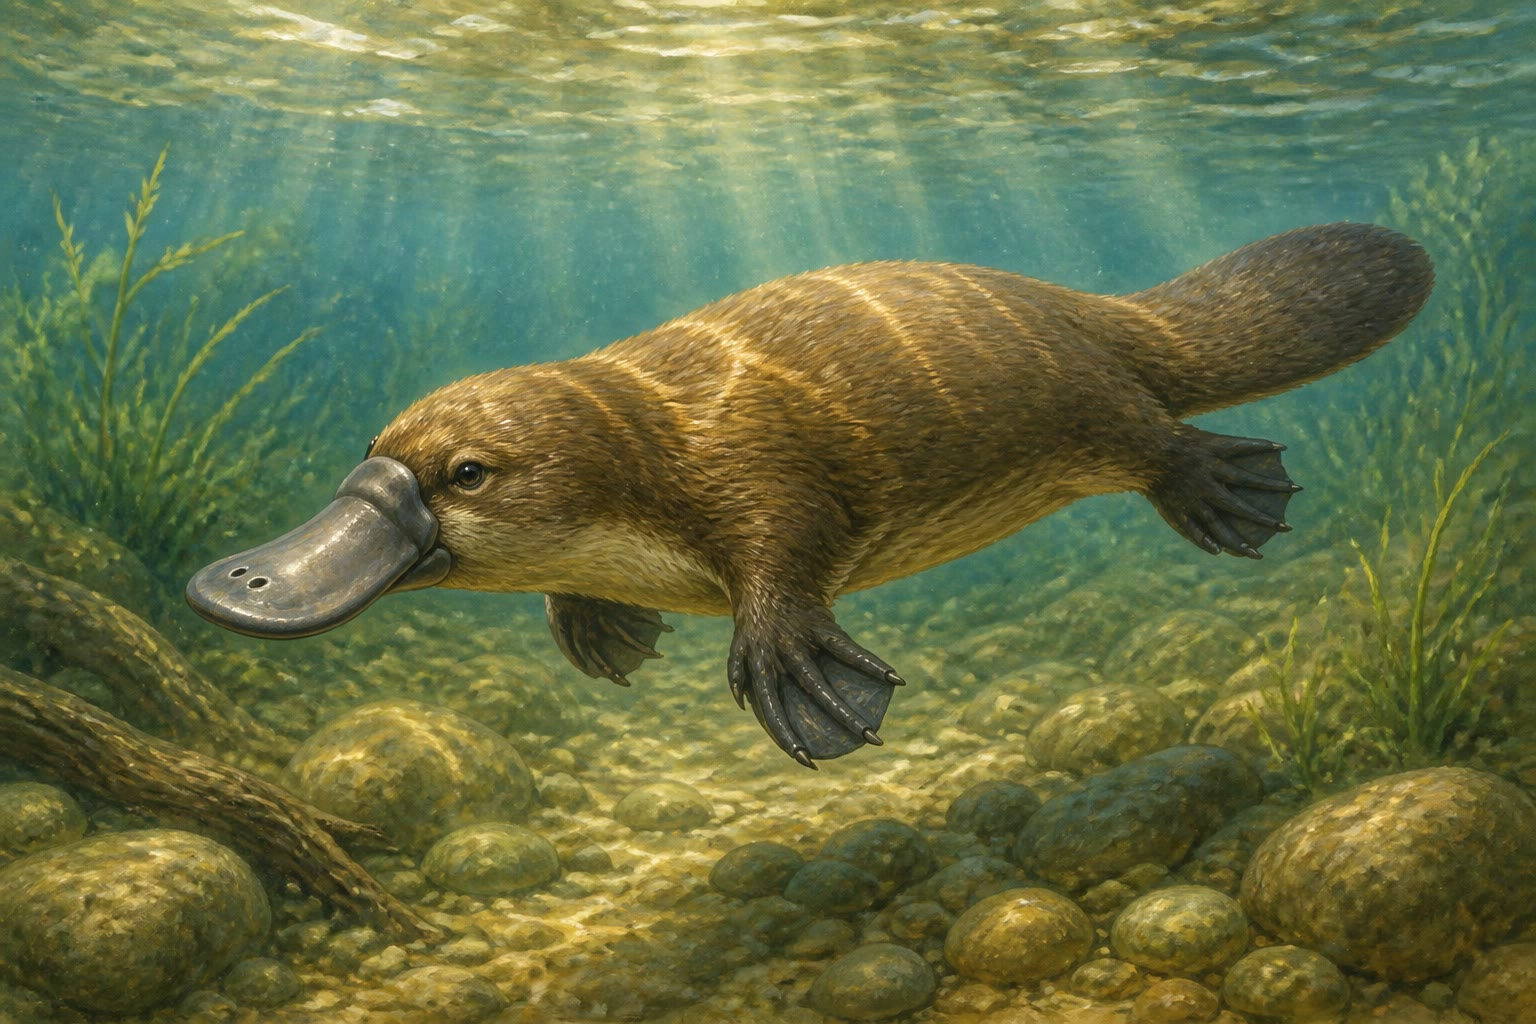
\includegraphics[width=0.6\linewidth]{images/book1/ai/g4-classify-platypus.jpg}

{\small \omterm{def:g4:classifying-animals:classification}{分类}学家最头疼的难题：有\omterm{def:g1:animals-around-us:covering}{皮毛}和\omterm{def:g2:animals-grow-up:born}{乳汁}，却有
喙、蹼足——还会产卵。鸭嘴兽（见最后一道
练习）检验了整个方法。}
\end{omfigure}

\section{练习}

\begin{exercise}[$\star$]\label{exo:g4:classifying-animals:1}
什么是\omterm{def:g4:classifying-animals:vertebrate}{脊椎动物}？什么是\omterm{def:g4:classifying-animals:vertebrate}{无脊椎动物}？
各举两个例子。
\end{exercise}

\begin{exercise}[$\star$]\label{exo:g4:classifying-animals:2}
写出五个\omterm{def:g4:classifying-animals:vertebrate}{脊椎动物}纲的名称，并给出各自的
主要特征。
\end{exercise}

\begin{exercise}[$\star$]\label{exo:g4:classifying-animals:3}
将下列\omterm{def:g1:animals-around-us:animal}{动物}分别归类：沙丁鱼、鳄鱼、蝾螈、
鸵鸟、鲸、蚯蚓。
\end{exercise}

\begin{exercise}[$\star$]\label{exo:g4:classifying-animals:4}
写出猫的层层嵌套“地址”，从最小的框到最大的框，
参照\cref{ex:g4:classifying-animals:cat}。
\end{exercise}

\begin{exercise}[$\star$]\label{exo:g4:classifying-animals:5}
蜥蜴和蝾螈外形相似。哪两项特征
能区分它们所属的纲？
\end{exercise}

\begin{exercise}[$\star$]\label{exo:g4:classifying-animals:6}
哪一个类群包含了绝大多数\omterm{def:g1:animals-around-us:animal}{动物}？
请列举其中四种成员。
\end{exercise}

\begin{exercise}[$\star$]\label{exo:g4:classifying-animals:7}
请大声逐题运行\cref{met:g4:classifying-animals:place}，
分别用于企鹅和海豚。
\end{exercise}

\begin{exercise}[$\star$]\label{exo:g4:classifying-animals:8}
只被告知：“这种\omterm{def:g1:animals-around-us:animal}{动物}是\omterm{prop:g3:sorting-living-things:groups}{鸟类}。”
请依据
\cref{prop:g4:classifying-animals:free}，列出三件你无需观察就能预料到的事。
\end{exercise}

\begin{exercise}[$\star\star$]\label{exo:g4:classifying-animals:9}
鲸几乎没有毛发，生活方式也像鱼。
运用\cref{met:g4:classifying-animals:place}和
\cref{ex:g3:sorting-living-things:surprises}，解释为何它仍是\omterm{prop:g3:sorting-living-things:groups}{哺乳动物}
——以及为何“生活在海里”从来
不是\omterm{def:g4:classifying-animals:classification}{分类}特征。
\end{exercise}

\begin{exercise}[$\star\star$]\label{exo:g4:classifying-animals:10}
蛇没有腿，蚯蚓也没有。为什么两者
一个是爬行类\omterm{def:g4:classifying-animals:vertebrate}{脊椎动物}，另一个是\omterm{def:g4:classifying-animals:vertebrate}{无脊椎动物}？哪一个单一特征
比缺少腿更具决定性？
\end{exercise}

\begin{exercise}[$\star\star\star$]\label{exo:g4:classifying-animals:11}
鸭嘴兽曾让博物学家大伤脑筋：有\omterm{def:g1:animals-around-us:covering}{皮毛}和\omterm{def:g2:animals-grow-up:born}{乳汁}，
却产下有壳的卵。哪一个纲占了上风，为什么？这个谜题
说明了按\emph{特征组合}而不是
按单一特征\omterm{def:g4:classifying-animals:classification}{分类}，有何启示？
\end{exercise}
